
\chapter{Permian Basin Background}
\label{CHAP:2}


%1. Oil and gas production from horizontal drilling and fracking
%2. Induced seismicity
%1. different theories of causes 
%2. difficulty in the Delaware basin case due to density
%3. Difficulty of observing subsurface changes


The Permian Basin has provided oil and gas from conventional reservoirs since the early 1900s (cite? frohlich?).
(Figure: Conventional vs EOR)

The turning point was around 2008 when companies began ...implementing? horizontal drilling and hydraulic fracturing, which opening up previously unproductive tight shale reservoirs.
(Figure of jump in productions)

% SmyeVariations
%Future development of the Wolfcamp A and B units in the Midland and Delaware Basins is expected to gen- erate $300 billion bbl of produced water, which will require man- agement of some type (Scanlon et al., 2020). More than 30 billion bbl of wastewater have been disposed throughout the Permian Basin, and disposal volumes have increased steadily since 2010 (Lemons et al., 2019)


During this time period, an increase in low magnitude earthquakes was observed. While West Texas had few seismic monitoring stations set up, one array near Lajitas, TX had been operating since 2000 \cite{Frohlich2019OnsetCauseIncreased}.


...as well as from geothermal energy development in locations such as Basel, Switzerland, where earthquakes were felt in 2006-2008. \cite{Deichmann2009EarthquakesInducedStimulation}.


There are many plausible physical models for how oil and gas production and wastewater injection may induce earthquakes along existing faults.
Spatiotemporal models have linked hydraulic fracturing to certain earthquakes \citep{Savvaidis2020InducedSeismicityDelaware}, (OTHER PAPER? ), but there has not been others .

%Earthquakes are triggered when the applied shear stress is greater than the critical stress τ#$%&
%Pressure from wastewater injection may play a role in certain areas (find that citation). This increasing of subsurface pore pressure could cause surface uplift in certain cases, and an example of this was reported on a single injection well (and single CO2 injection?) by \cite{Kim2018AssociationLocalizedGeohazards}.s

Something about the CMEZ. maybe look into Peter/lilly for fauly mapping, maybe something from Katie?

Check how the recent eq papers 

TODO: need to look into recent mentone stuff. peters papers, recent skoumal paper



The success of shale development technologies \citep{Waters2006Spe103202Ms} has opened up vast shale resources for economically viable oil and gas production. Based on a recent assessment by the U.S. Geological Survey (USGS), the Wolfcamp shale in Texas' Permian Basin is the largest continuous oil field that has ever been discovered in the United States \citep{GaswirthAssessment2016} . As of 2017, there were over 130,000 active production wells, 23,041 active enhanced oil production (EOR) wells, and 3794 active saltwater disposal (SWD) wells in the Permian Basin (Figure \ref{fig:permian-oil-6panel} (a)). It has been recognized that injection or withdrawal of fluids from the subsurface can induce earthquakes along existing faults \citep{Ellsworth2013, simpson1988two}. While petroleum production and wastewater injection volumes have been rising throughout the basin, the recently cataloged earthquakes are spatially clustered (Figure \ref{fig:Permian} (b)-(f)). One significant cluster is near Pecos, TX, where increased seismic activity began in 2009. Subsequent activity has increased considerably, with more than 2000 earthquakes identified in 2017 \citep{Frohlich2019}.




\begin{figure}[hbt!]
	\centering
	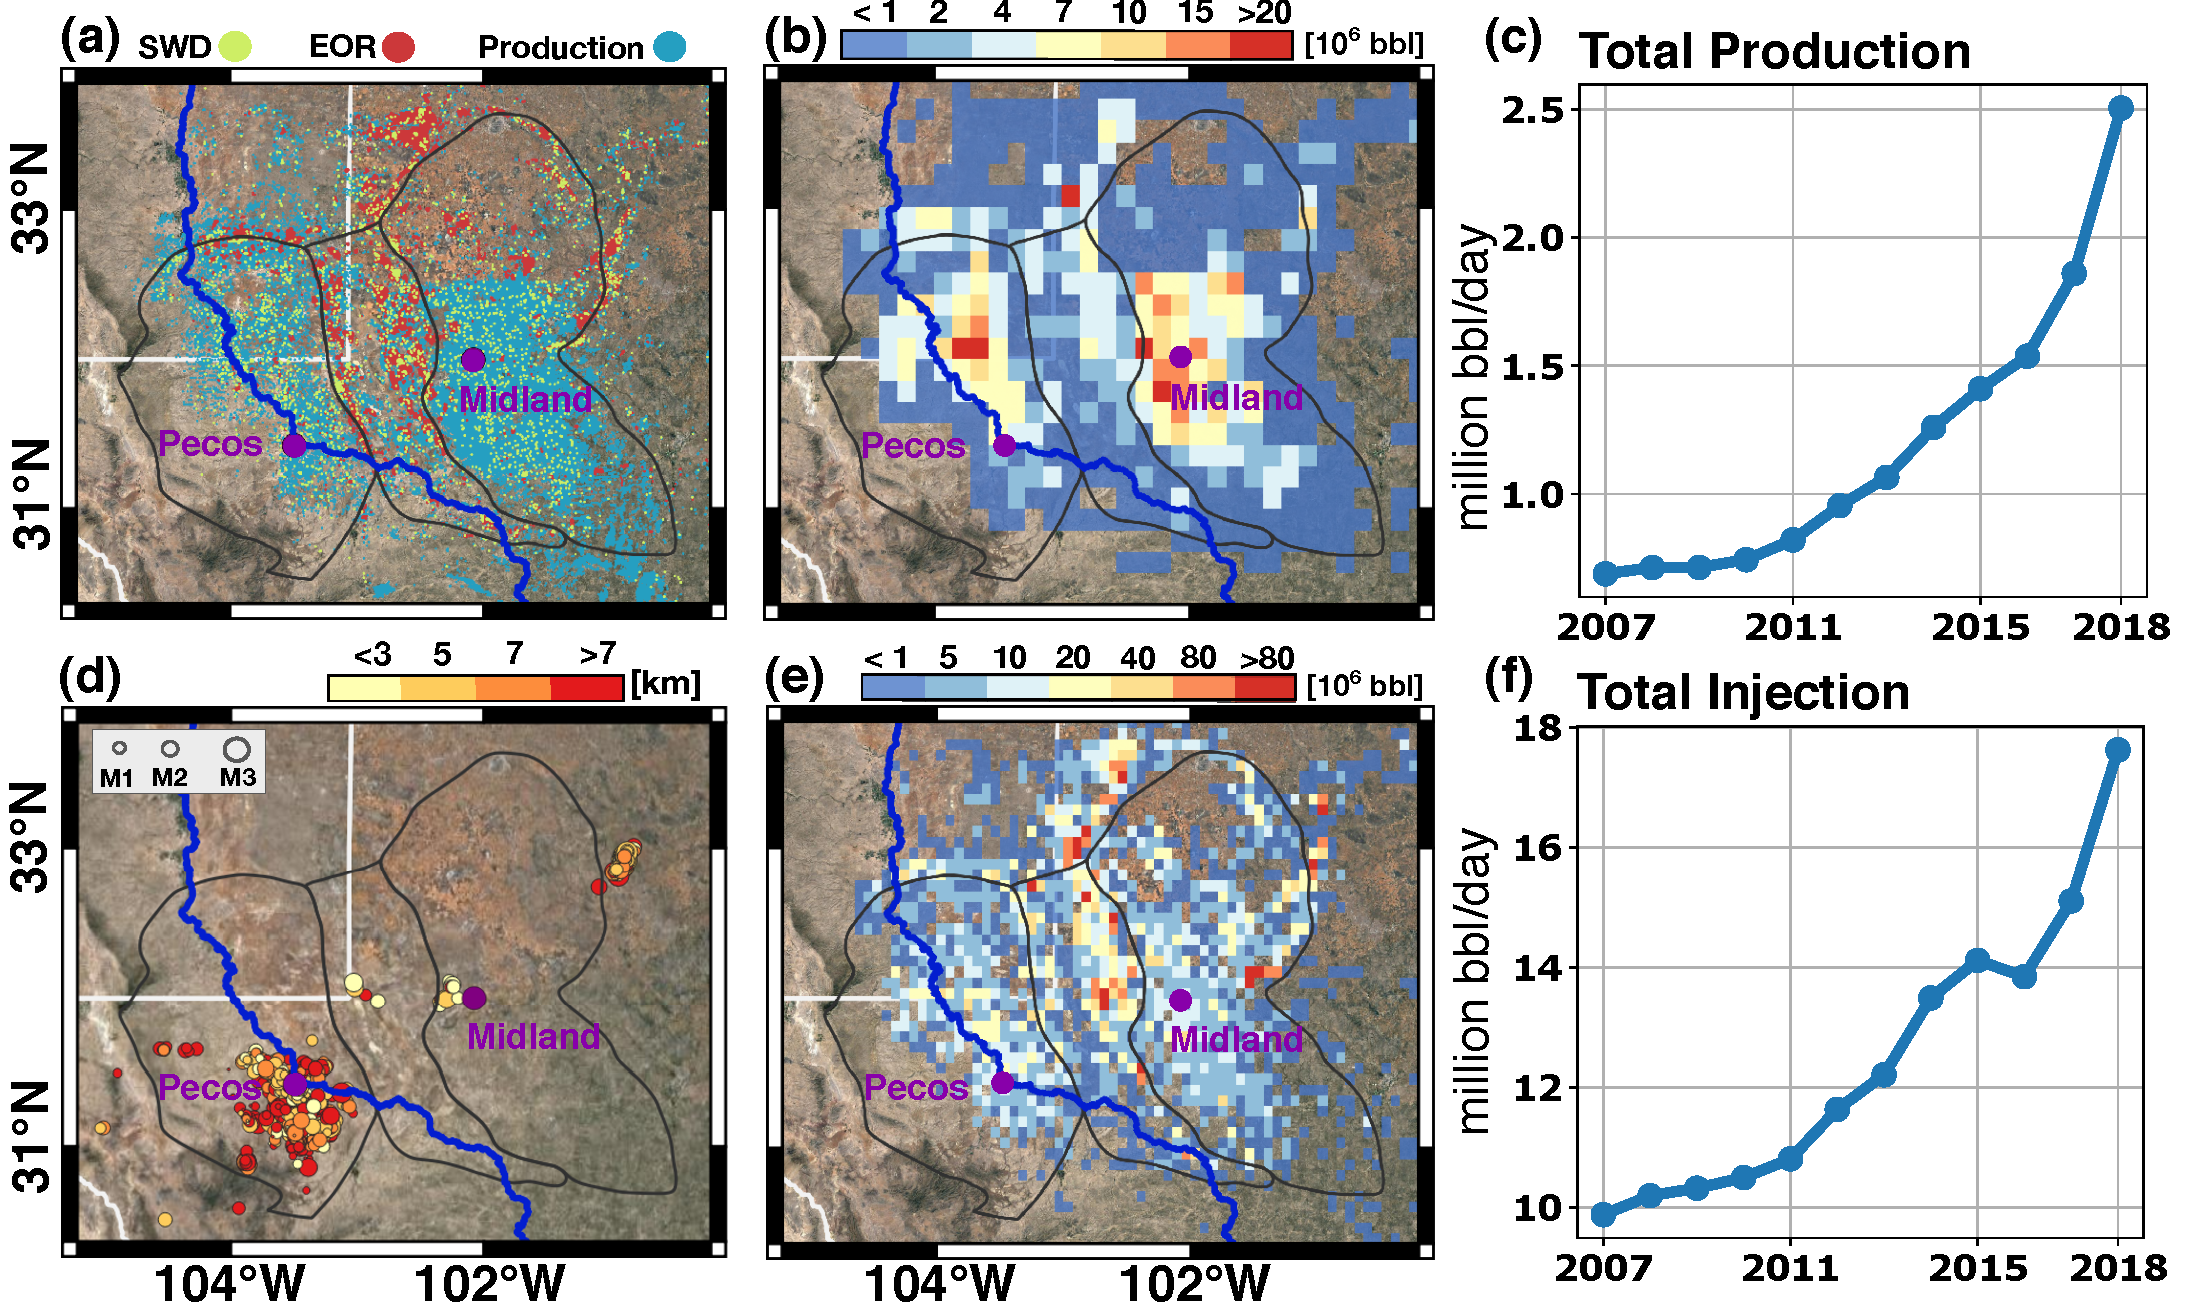
\includegraphics[width=0.99\linewidth]{paper1-permian/figures/supplement/figureS1-cisr-data.pdf}
	\caption[Shale development and induced seismicity in the Permian Basin.]{Shale development and induced seismicity in the Permian Basin. 
		(a) Locations of oil production, enhanced oil recovery (EOR), and saltwater disposal (SWD) wells active in 2017. (b) Annual oil production volume on a 10-mile grid in 2017. (c) Permian region oil production rate as reported by the Texas Railroad Commission. (d) Locations of earthquake hypocenters detected by TexNet in 2017. The color and size of a circle indicates the estimated earthquake depth and magnitude. (e) Annual injection volume (including both SWD and EOR wells) on a 5-mile grid. (f) Permian region injection rate (including both SWD and EOR wells) as reported by the Texas Railroad Commission.
	}
	\label{fig:permian-oil-6panel}
\end{figure}


Understanding the nature and causes of earthquakes and how they are linked to certain production and disposal wells requires extensive knowledge of the subsurface. InSAR surface deformation measurements allow us to estimate the distribution of fault slip at depth and infer the associated seismic risk \citep{Segall2010, huang2017fault}. Furthermore, measurements of reservoir inflation due to wastewater injection allows operators to assess pressure build-up in disposal aquifers and the associated triggered seismicity risk. It is also worth noting that oil recovery in shale wells is notoriously low \citep{clark2009determination}, and the performance of these wells varies significantly. InSAR can be employed to map subsurface fluid depletion and pressurization. These surface deformation observations, when coupled with reservoir compaction inversion modeling, can be used to assess the areal effectiveness of oil and gas extraction operations \citep{Du2001, Vasco2005}. 
mechanically layered earth as a homogeneous half space, even though the stiffness increases with depth \citep{Du1992}. 

